Prije nego što počnemo govoriti o samom programskom jeziku valjalo bi napomenuti da je Java zapravo i programski jezik i platforma. Neke osnovne informacije o Java programskom jeziku i samoj Java platformi je potrebno znati prije nego što se upustimo u programiranje Java aplikacija.

\section{Programski jezik Java}
Slika~\ref{fig:software-development-process} prikazuje pregled procesa razvoja Java aplikacije.
\begin{figure}[h!]
    \label{fig:software-development-process}
    \caption{Proces razvoja Java aplikacije.}
    \centering
    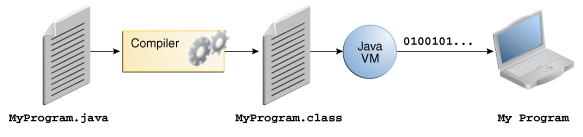
\includegraphics[width=\textwidth]{images/software-development-process}
\end{figure}

U Java programskom jeziku, izvorni kôd (eng. \emph{source code}) je pisan u tekstualnim datotekama. Nazivi tih datoteka završavaju sa .java.

No te datoteke su pisane od strane programera i one, kao takve, nisu razumljive samom procesoru računala kojeg želimo isprogramirati. Taj problem rješava Java prevoditelj (eng. \emph{compiler}) koji će uzeti te datoteke koje su napisane od strane programera i prevesti ih u oblik razumljiv računalu. Dakle, za svaku datoteku koja sadrži izvorni kôd će napraviti po jednu dodatnu datoteku istog naziva samo drugačijeg završetka - \texttt{.class}. Drugim riječima, ako imamo datoteku naziva \texttt{MyProgram.java} tada će prevoditelj proizvesti datoteku naziva \texttt{MyProgram.class}. Postupak prevođenja datoteke koja sadrži izvorni kôd u datoteku koja sadrži Java \emph{bytecode} je opisan sljedećim primjerom: Ako postoji izvorni kôd napisan u \texttt{MyProgram.java} datoteci koju želimo prevesti u \texttt{MyProgram.class} datoteku koja sadrži Java \emph{bytecode} onda moramo u naredbenom retku upisati sljedeće:

\begin{lstlisting}
$ javac MyProgram.java
\end{lstlisting}
